\documentclass[border=2pt]{standalone}
\usepackage{tikz,amsmath}
\begin{document}
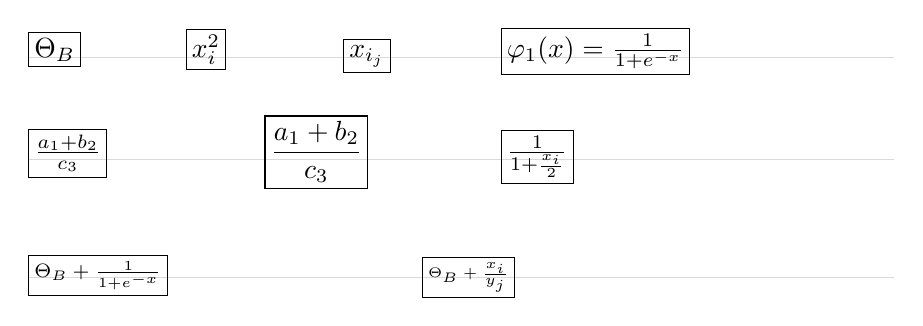
\begin{tikzpicture}
  \draw[gray!30] (0,0)--(11,0) (0,-1.3)--(11,-1.3) (0,-2.8)--(11,-2.8);
  \node[anchor=base west,draw,inner sep=2pt] at (0,0) {$\Theta_B$};
  \node[anchor=base west,draw,inner sep=2pt] at (2,0) {$x_i^2$};
  \node[anchor=base west,draw,inner sep=2pt] at (4,0) {$x_{i_j}$};
  \node[anchor=base west,draw,inner sep=2pt] at (6,0) {$\varphi_1(x)=\frac{1}{1+e^{-x}}$};
  \node[anchor=base west,draw,inner sep=2pt] at (0,-1.3) {$\frac{a_1+b_2}{c_3}$};
  \node[anchor=base west,draw,inner sep=2pt] at (3,-1.3) {$\dfrac{a_1+b_2}{c_3}$};
  \node[anchor=base west,draw,inner sep=2pt] at (6,-1.3) {$\frac{1}{1+\frac{x_i}{2}}$};
  \node[anchor=base west,draw,inner sep=2pt,font=\scriptsize] at (0,-2.8) {$\Theta_B+\frac{1}{1+e^{-x}}$};
  \node[anchor=base west,draw,inner sep=2pt,font=\tiny] at (5,-2.8) {$\Theta_B+\frac{x_i}{y_j}$};
\end{tikzpicture}
\end{document}
